% Version 1.0 January 2009
%
% To compile to pdf, run:
% latex plos.template
% bibtex plos.template
% latex plos.template
% latex plos.template
% dvipdf plos.template

\documentclass[12pt]{article}\usepackage[]{graphicx}\usepackage[]{color}
%% maxwidth is the original width if it is less than linewidth
%% otherwise use linewidth (to make sure the graphics do not exceed the margin)
\makeatletter
\def\maxwidth{ %
  \ifdim\Gin@nat@width>\linewidth
    \linewidth
  \else
    \Gin@nat@width
  \fi
}
\makeatother

\definecolor{fgcolor}{rgb}{0.345, 0.345, 0.345}
\newcommand{\hlnum}[1]{\textcolor[rgb]{0.686,0.059,0.569}{#1}}%
\newcommand{\hlstr}[1]{\textcolor[rgb]{0.192,0.494,0.8}{#1}}%
\newcommand{\hlcom}[1]{\textcolor[rgb]{0.678,0.584,0.686}{\textit{#1}}}%
\newcommand{\hlopt}[1]{\textcolor[rgb]{0,0,0}{#1}}%
\newcommand{\hlstd}[1]{\textcolor[rgb]{0.345,0.345,0.345}{#1}}%
\newcommand{\hlkwa}[1]{\textcolor[rgb]{0.161,0.373,0.58}{\textbf{#1}}}%
\newcommand{\hlkwb}[1]{\textcolor[rgb]{0.69,0.353,0.396}{#1}}%
\newcommand{\hlkwc}[1]{\textcolor[rgb]{0.333,0.667,0.333}{#1}}%
\newcommand{\hlkwd}[1]{\textcolor[rgb]{0.737,0.353,0.396}{\textbf{#1}}}%

\usepackage{framed}
\makeatletter
\newenvironment{kframe}{%
 \def\at@end@of@kframe{}%
 \ifinner\ifhmode%
  \def\at@end@of@kframe{\end{minipage}}%
  \begin{minipage}{\columnwidth}%
 \fi\fi%
 \def\FrameCommand##1{\hskip\@totalleftmargin \hskip-\fboxsep
 \colorbox{shadecolor}{##1}\hskip-\fboxsep
     % There is no \\@totalrightmargin, so:
     \hskip-\linewidth \hskip-\@totalleftmargin \hskip\columnwidth}%
 \MakeFramed {\advance\hsize-\width
   \@totalleftmargin\z@ \linewidth\hsize
   \@setminipage}}%
 {\par\unskip\endMakeFramed%
 \at@end@of@kframe}
\makeatother

\definecolor{shadecolor}{rgb}{.97, .97, .97}
\definecolor{messagecolor}{rgb}{0, 0, 0}
\definecolor{warningcolor}{rgb}{1, 0, 1}
\definecolor{errorcolor}{rgb}{1, 0, 0}
\newenvironment{knitrout}{}{} % an empty environment to be redefined in TeX

\usepackage{alltt}

\usepackage{amsmath, amssymb, graphicx, color, enumerate, float}

% Use doublespacing - comment out for single spacing
%\usepackage{setspace} 
%\doublespacing

\usepackage{dcolumn}

% Text layout
\topmargin 0.0cm
\oddsidemargin 0.5cm
\evensidemargin 0.5cm
\textwidth 16cm 
\textheight 21cm

\usepackage{ifxetex}
\ifxetex
%\usepackage{fontspec}
  \usepackage{unicode-math}
  \setmathfont{[Asana-Math]}
\fi

\usepackage[
  natbib = true,
    backend=bibtex,
    isbn=false,
    url=false,
    doi=false,
    eprint=false,
    style=numeric-comp,
    sorting=none,
    sortcites = true,
    firstinits=true,
    terseinits=true,
    date=year,
	maxbibnames=6, minbibnames=6
  ]{biblatex}

\renewcommand*{\multicitedelim}{\addcomma}


%\renewcommand*{\revsdnamepunct}{}


\renewbibmacro{in:}{\ifentrytype{article}{}{\printtext{\bibstring{in}\intitlepunct}}}

\DeclareFieldFormat[article,incollection,book,inbook,inproceedings]{pages}{#1}

\newif\ifseverity
\severitytrue
%\severityfalse


\DeclareFieldFormat[article,inbook,incollection,inproceedings,patent,thesis,unpublished]{citetitle}{#1}
\DeclareFieldFormat[article,inbook,incollection,inproceedings,patent,thesis,unpublished]{title}{#1} 


\DeclareFieldFormat{titlecase}{\MakeTitleCase{#1}}

\newrobustcmd{\MakeTitleCase}[1]{%
  \ifthenelse{\ifcurrentfield{booktitle}\OR\ifcurrentfield{booksubtitle}%
    \OR\ifcurrentfield{maintitle}\OR\ifcurrentfield{mainsubtitle}%
	\OR\ifcurrentfield{journaltitle}\OR\ifcurrentfield{journalsubtitle}%
	\OR\ifcurrentfield{issuetitle}\OR\ifcurrentfield{issuesubtitle}%
    \OR\ifentrytype{book}\OR\ifentrytype{mvbook}\OR\ifentrytype{bookinbook}%
    \OR\ifentrytype{booklet}\OR\ifentrytype{suppbook}%
    \OR\ifentrytype{collection}\OR\ifentrytype{mvcollection}%
    \OR\ifentrytype{suppcollection}\OR\ifentrytype{manual}%
    \OR\ifentrytype{periodical}\OR\ifentrytype{suppperiodical}%
    \OR\ifentrytype{proceedings}\OR\ifentrytype{mvproceedings}%
    \OR\ifentrytype{reference}\OR\ifentrytype{mvreference}%
    \OR\ifentrytype{report}\OR\ifentrytype{thesis}}
    {#1}
    {\MakeSentenceCase{#1}}}

   %%
    
    
\DeclareFieldFormat{journaltitle}{\mkbibemph{#1\adddot}}



%%%%%%%%%%%%%%%%%%%%%%%%%%%%%%%%%%%

% Comma before date; date not in parentheses
\newbibmacro*{year+volume+pages}{%
	\printfield{year}
	  \setunit*{\addsemicolon}%
	\printfield{volume}
	  \newunit
	\setunit*{\addcolon}
	\printfield{pages}
  \newunit}

% Issue/date macros removed after journal number
\renewbibmacro*{journal+issuetitle}{%
  \usebibmacro{journal}%
  \newunit}

% "In:" removed for articles; issue/date macros added after note+pages macro
\DeclareBibliographyDriver{article}{%
  \usebibmacro{bibindex}%
  \usebibmacro{begentry}%
  \usebibmacro{author/translator+others}%
  \setunit{\labelnamepunct}\newblock
  \usebibmacro{title}%
  \newunit
  \printlist{language}%
  \newunit\newblock
  \usebibmacro{byauthor}%
  \newunit\newblock
  \usebibmacro{bytranslator+others}%
  \newunit\newblock
  \printfield{version}%
  \newunit\newblock
%  \usebibmacro{in:}% DELETED
  \usebibmacro{journal}%
  \newunit
  \usebibmacro{byeditor+others}%
  \newunit
  \usebibmacro{year+volume+pages}%
  \newunit\newblock
  \iftoggle{bbx:isbn}
    {\printfield{issn}}
    {}%
  \newunit\newblock
  \usebibmacro{addendum+pubstate}%
  \setunit{\bibpagerefpunct}\newblock
  \usebibmacro{pageref}%
  \usebibmacro{finentry}}
  
  
  %  Inproceedings changes
\newbibmacro*{publisher+location+date}{%
	\printlist{publisher}
	\setunit*{\adddot\space}
	\printfield{location}
	\setunit*{\adddot\space}
	\printfield{year}
	\setunit*{\addsemicolon}%
	\printfield{volume}
	\newunit
	\setunit*{\addcolon}
	\printfield{pages}
  \newunit}
  
\DeclareFieldFormat[inproceedings]{volume}{#1}
  
\DeclareBibliographyDriver{inproceedings}{%
  \usebibmacro{bibindex}%
  \usebibmacro{begentry}%
  \usebibmacro{author/translator+others}%
  \setunit{\labelnamepunct}\newblock
  \usebibmacro{title}%
  \newunit
  \printlist{language}%
  \newunit\newblock
  \usebibmacro{byauthor}%
  \newunit\newblock
  \usebibmacro{bytranslator+others}%
  \newunit\newblock
  \printfield{version}%
  \newunit\newblock
  \usebibmacro{in:}% DELETED
  \usebibmacro{booktitle}%
  \newunit
  \usebibmacro{publisher+location+date}%
  \newunit\newblock
  \iftoggle{bbx:isbn}
    {\printfield{issn}}
    {}%
  \newunit\newblock
  \usebibmacro{addendum+pubstate}%
  \setunit{\bibpagerefpunct}\newblock
  \usebibmacro{pageref}%
  \usebibmacro{finentry}}
    
%%%%%%%%%%%%%%%%%%%%%%%%%%%%%%%%%%%

\DeclareNameAlias{sortname}{last-first}
\DeclareNameAlias{default}{last-first}



  
%\bibliography{CT_Pipeline_l}
%\bibliography{extra_pubs}

\addbibresource{CT_Pipeline_l}
\addbibresource{extra_pubs}



% Bold the 'Figure #' in the caption and separate it with a period
% Captions will be left justified
\usepackage[labelfont=bf,labelsep=period,justification=raggedright,tableposition=bottom]{caption}

% Use the PLoS provided bibtex style

% Remove brackets from numbering in List of References
\newcommand{\bbeta}{\mbox{\boldmath $\beta$}}

% Leave date blank
\date{}
\pagestyle{myheadings}
% \usepackage{natbib}
\usepackage{subfig}
\usepackage{hyperref}
\graphicspath{{maps/}}
\renewcommand{\thesubfigure}{\Alph{subfigure}}
\IfFileExists{upquote.sty}{\usepackage{upquote}}{}
\begin{document}
\begin{refsection} % refsection environment
\pagenumbering{gobble}% Remove page numbers (and reset to 1)
\thispagestyle{empty}
%All authors have read and approved the submitted manuscript, the manuscript has not been submitted elsewhere nor published elsewhere in whole or in part.

\newpage 
%\section*{Title Page}
\begin{flushleft}
{\Large
\textbf{Quantitative Localization of Supratentorial Intracranial Hemorrhage}
}
\\
John Muschelli$^{1,\ast}$, ScM;
Natalie L. Ullman$^{2}$, BS;
Elizabeth M. Sweeney$^{1}$, ScM;
Ani Eloyan$^{1}$, PhD; 
Neil Martin$^{3}$, MD;
Paul Vespa$^{3}$, MD;
Daniel F. Hanley$^{2}$, MD;
Ciprian M. Crainiceanu$^{1}$, PhD
\\
\bf{1} Department of Biostatistics, Bloomberg School of Public Health, Johns Hopkins University, Baltimore, MD
\\
\bf{2} Department of Neurology, Division of Brain Injury Outcomes,  Johns Hopkins Medical Institutions, Baltimore, MD
\\
\bf{3} Department of Neurosurgery, David Geffen School of Medicine at UCLA, Los Angeles, CA
\\
%\bf{4} Section of Neurosurgery and the Neurovascular Surgery Program, University of Chicago Pritzker School of Medicine, Chicago, IL
%\\
$\ast$ E-mail: jmusche1@jhu.edu
\end{flushleft}



\newpage 






























% Please keep the abstract between 250 and 300 words
\section*{Abstract}


\subsection*{Background and Purpose}
Standard radiologic description of intracranial hemorrhage (ICH) location is subjective and qualitative.  Using registration of computed tomography (CT) brain images, we provide objective, detailed quantification of ICH location.

\subsection*{Methods}
We analyzed images from patients ($N{=}111$) enrolled in the MISTIE (Minimally Invasive Surgery plus recombinant-tissue plasminogen activator for Intracerebral Evacuation) trial.  We registered CT scans to a CT template, estimated a 3-dimensional map of ICH engagement location, and estimated areas of ICH engagement. 

\subsection*{Results}
In this sample, ICH primarily located in deep brain nuclei and lobar white matter, including the insula, superior temporal gyrus, and the putamen.

\subsection*{Conclusions}
Objective measures of ICH location and engagement using advanced CT imaging processing provide finer, objective, and more quantitative anatomic information than that provided by human readers. 

\subsection*{Clinical Trial Registration Information}
Clinical Trial Registration-URL: \url{http://www.clinicaltrials.gov}. Unique identifier: NCT00224770.


{\bf Keywords:} Intracerebral Hemorrhage; CT and MRI

\newpage

\section*{Introduction}

Intracranial hemorrhage (ICH) results from a blood vessel rupturing into brain tissues and possibly the ventricles. The classification and quantitative descriptions of hemorrhage location using X-ray computed tomography (CT) is complicated: it may extend into multiple brain areas, distend tissues, and break through the ventricular wall. Therefore, routine practice identifies one primary affected anatomic region (e.g.~caudate) \citep{mendelow_early_2013, anderson_intensive_2008, antihypertensive_treatment_of_acute_cerebral_hemorrhage_atach_investigators_antihypertensive_2010} or describes the hemorrhage in relation to a landmark \citep{ziai_multicenter_2014}.

Detailed localization information can be obtained, however, by registering scans to a common template where labeled brain atlases are available. After registration, each patient scan is located in the same stereotaxic template space so information may be combined spatially across scans. We registered CT images to a previously-published CT template \citep{rorden_age-specific_2012}, located in MNI (Montreal Neurological Institute) space, using the provided software. 

Our goal is to quantitatively and objectively characterize ICH location\ifseverity
, compare this characterization to human labeling, and predict stroke severity scores using ICH location information. 
\else
.
\fi


\section*{Methods}

To achieve this goal, we 1) created a 3-dimensional (3D) density map of supratentorial hemorrhages\ifseverity
, 
\else
 and 
\fi 2) provided detailed quantification of hemorrhage engagement of individual neuroanatomic regions\ifseverity
, 3) performed voxel-wise tests of ICH location on 2 severity scores: Glasgow Coma Scale (GCS) and National Institutes of Health Stroke Scale (NIHSS) and 4) summarized significantly predictive voxel regions into patient-level covariates.
\else 
.
\fi



\subsection*{Subjects and Demographics}
The population studied consists of 111 patients from the MISTIE (Minimally Invasive Surgery plus recombinant-tissue plasminogen activator for Intracerebral Evacuation) \citep{morgan_preliminary_2008} trial recruited from 26 centers with lobar and deep ICHs $\geq$20mL in volume.    This sample was $31.5$\% female with mean (SD) age of 60.8 (11.2) years.

% Descriptive demographics of age, sex, race, and baseline ICH and intraventricular hemorrhage (IVH) volumes are shown in Table~\ref{t:dem}.  

% CT and clinical data were collected as part of the Johns Hopkins Medicine IRB-approved MISTIE research studies with written consent from participants. 

\thickmuskip=0mu

\subsection*{Imaging Data}
Standard diagnostic CT images were acquired under a standard protocol but with differences across sites.  Scans were acquired using GE ($N{=}46$), Siemens ($N{=}37$), Philips ($N{=}20$), and Toshiba ($N{=}8$) scanners, had gantry tilt ($N{=}87$), and the slice thickness of the image varied within some scans ($N{=}14$). Therefore, the scans analyzed had different voxel (volume element) dimensions and image resolution prior to registration to the template. 
%These conditions represent a pragmatic sample of stroke center diagnostic imaging.
\thickmuskip=5mu plus 5mu


\subsection*{Hemorrhage Segmentation and Location Identification}
ICH was manually segmented using the OsiriX (v.4.1, Pixmeo; Geneva, Switzerland) by expert readers.  Readers employed a semi-automated approach: a Hounsfield unit range of $40$ to $80$ selected potential regions of ICH \citep{bergstrom_variation_1977, smith_imaging_2006}, then these regions were manually adjusted. Readers identified the anatomic location most engaged by the ICH: putamen ($N{=}68$), lobar ($N{=}33$), globus pallidus ($N{=}6$), and thalamus ($N{=}4$).  The initial mean (SD) ICH volume of this sample was 37.4 (20.1) mL.


\subsection*{Image Registration}
The brain image was spatially registered to the CT template using the Clinical toolbox \citep{rorden_age-specific_2012} and the statistical parametric mapping software (SPM8, Wellcome Trust Centre for Neuroimaging, London, UK) in MATLAB (Mathworks, Natick, Massachusetts, USA).  The binary hemorrhage mask was transformed into the template space. No scans were excluded due to inadequate registration, determined by visual inspection.


\subsection*{ICH Localization and Engagement}
\label{sec:engage}
We estimated a 3D histogram of ICH localization: for every voxel in template space, we calculated the proportion of patients who have an ICH at that particular voxel.  
 
%Although prediction of severity score is of interest, standard practice conveys information based on known neuroanatomic regions.  
We calculated spatial ICH engagement by neuroanatomic region using the ``Eve" atlas \citep{oishi_human_2008}, which segments gray matter (GM) and white matter (WM) regions.  
Ventricular regions were not explicitly segmented in the Eve atlas.  Any region not classified was reported as cerebrospinal fluid (CSF).


From this atlas, we estimated ICH engagement at the population level: 1) the percent of the ICH engaged by region (e.g.~putamen engages 20\% of the ICH) and 2) the percent of each region engaged by the ICH (e.g.~ICH engages 78\% of the putamen).  These summaries of ICH engagement provide a finer description than one location (e.g.~putamen).  

\ifseverity
In the study population, 1,045,174 voxels (denoted by $V$) had at least one patient with ICH.  We limited our analysis to voxels in the template space where at least 10 patients exhibit ICH (166,202 voxels) to optimize the models for a substantial proportion of the study population.

We tested the association between hemorrhage location and stroke severity by running voxel-wise t-tests, testing the null hypothesis $H_{0}(v):\mu_{1}(v)=\mu_{0}(v)$, where $\mu_{1}(v)$ corresponds to the mean score (NIHSS or GCS) in patients where $ICH{=}1$ at voxel $v$, similarly for $\mu_{0}(v)$. 


We created a patient-level covariate that summarizes ICH location information by selecting regions using a sequence of nested p-value thresholds.  We call these regions ``highest predictive regions'' (HPR) because they contain the voxels that are most predictive of the severity scores. 
We obtained $6$ different HPR, $3$ based on the smallest $1000$, $2000$, or $3000$ lowest p-values and three based on p-values thresholds of $.05$, $.01$, and $.001$. For each HPR, we calculated the HPR ``coverage" for scan $i$: 
$$
\text{HPR Coverage}_i = \frac{\text{\# Voxels classified ICH in HPR for scan } i}{\text{\# Voxels in HPR}} \times 100\% \nonumber
$$
and used this as a predictor of the severity score ($Y_i$), adjusting for age, sex, and baseline ICH volume (ICHVol):
\begin{equation}
{\rm Y}_i = \beta_0 + \beta_1 {\rm Coverage}_i + \gamma_1{\rm Age}_i  +\gamma_2{\rm Sex}_i +\gamma_3{\rm ICHVol}_i + \epsilon_{i} \label{eq:cov}
\end{equation}
\thickmuskip=0mu
We compared model~\eqref{eq:cov} using adjusted $R^2$ to one using a categorical indicator of the expert-specified ICH location, with categories: thalamus, globus pallidus, putamen, and lobar.  
A permutation test was used: the severity score was randomly permuted, the HPR was estimated, and the adjusted $R^2$ was calculated. The p-value was obtained by comparing the distribution of permuted adjusted $R^2$ with the estimated adjusted $R^2$ from the HPR model. 
\fi
\section*{Results}

\subsection*{Prevalence of ICH Engagement in the Brain}

Figure~\ref{fig:StrokeHist} represents the 3D histogram of hemorrhage prevalence, where colors represent the percentage of patients with ICH engagement at that voxel.  ICH is distributed medially in the brain in this cohort, with a lower concentration at the cortical surface and higher on the left side of the brain.   The majority of voxels have a low prevalence of ICH engagement; the median number of patients with ICH at a voxel is 3 (3\%), though some voxels ($V{=}5685$) have a high prevalence of ${>}40\%$ of the sample population.  


\thickmuskip=5mu plus 5mu

%***
%Combining regions of engagement from the left and right sides of the brain is worthwhile as regions will likely affect severity regardless of the hemisphere engaged. We did not combine these areas, as it may not be straightforward to combine ICH that crosses the mid-sagittal plane. We did attempt to ``symmetrize'' the HPR by including voxels regardless of the side of the brain.  If a voxel on the left side of the brain was included in the HPR, the corresponding voxel on the right side was included in the symmetrized HPR.  We observed similar patterns to Figure 3C and 3D using the symmetrized HPR  (see \url{http://stroke.ahajournals.org}).


\subsubsection*{ICH Localization and Engagement}
Table~\ref{t:breakdown} represents the 10 most-engaged regions for the population 3D histogram.  The engagement represents the percent engagement of a specific area compared to all areas engaged.  The 3D histogram of ICH is engaged in areas of the insula, putamen, and primarily the CSF (i.e.~ventricles and subarachnoid spaces). 

We also calculated the engagement of the thalamus, putamen, and globus pallidus by the population 3D histogram.  The population engagement represents the mean proportion of ICH prevalence in the population for that brain region.  On average, 23\% of the putamen, 20\% of the globus pallidus, and 8\% of the thalamus are engaged with ICH from patients in this study. 

Registering images with large deformations caused by the hemorrhage, even those using non-linear registration, will likely have mis-registration artifacts.  Lateral shift caused by the hemorrhage, resulting in compression of ventricles, may lead to mapping some areas of the hemorrhage or tissue to the ventricles in template space.  Combining multiple registration approaches may achieve better results.



\ifseverity
\subsubsection*{Highest Predictive Region Analysis}




\thinmuskip=0mu


For illustration, panel (\protect\subref*{pvals:nihss}) in Figure~\ref{f:roi} displays the region of p-values smaller than $.01$ for the voxel-wise t-tests of NIHSS and panel~(\protect\subref*{pvals:gcs}) displays voxels with the smallest $1000$ p-values testing GCS score. These regions were the HPR with the highest adjusted $R^2$ in \eqref{eq:cov}. We show three orthographic slices for each HPR; the entire regions are available in MNI coordinates. 
\thinmuskip=3mu

Figure~\ref{f:roi}\protect\subref*{pvals:regnihss} displays the NIHSS score as a function of the coverage of the HPR from Figure~\ref{f:roi}\protect\subref*{pvals:nihss}. Similarly, Figure~\ref{f:roi}\protect\subref*{pvals:reggcs} displays the GCS score as a function of the coverage of the HPR in Figure~\ref{f:roi}\protect\subref*{pvals:gcs}.  The blue line represents a non-parametric LOESS (local regression) \citep{cleveland_local_1992} fit and the red line represents an unadjusted linear model fit.  As expected, the larger the HPR coverage the higher (more severe stroke) the NIHSS score and the lower (deeper unconsciousness) the GCS score.

Adjusted $R^2$ model estimates indicated all HPR coverage models strongly outperform reader-classified location models: the adjusted $R^2$ almost doubled from $0.129$  for the reader-classified location model to $0.254$ for NIHSS; the adjusted $R^2$ more than tripled from $0.069$ for the reader-classified location model to $0.214$ for the HPR coverage model for GCS. 

The permutation test p-values were $<.001$ for HPR of NIHSS and $<.01$ for HPR of GCS, indicating that the selected HPRs were more predictive than HPRs obtained using the same selection procedure when there is no association between location and stroke severity scores. 
\fi

\section*{Discussion}

We have characterized the localization of ICH in a population from prospective clinical trial images using a 3D histogram. We found the well-described medial location of most supratentorial ICHs.   We can create 3D histograms based on subgroups or different study populations and test differences between groups at a voxel level using proportion tests, allowing a fine-scale comparison ICH location across groups.

We also demonstrate how labeled atlases can automatically describe ICH engagement by neuroanatomic regions at a patient or population level. These measures are more interpretable for clinical relevance and may translate to better determination of disability.


\subsection*{Summary}
The summary of Eve-atlas ICH engagement presented provided a finer description of location than previously possible by human readers. This type of analysis provides a framework for derivation and testing measures of ICH engagement.  We hope this method will engage others with larger data sets and methodological skills to enhance the use of quantitative localization. 



\section*{Sources of Funding}
The project described was supported by the grant RO1EB012547 (NIH), T32AG000247 (NIA), R01NS046309, RO1NS060910, RO1NS085211, R01NS046309, U01NS080824 and U01NS062851 (NINDS), and RO1MH095836 (NIMH).

\section*{Disclosures}
Johns Hopkins University holds a use patent for intraventricular tissue plasminogen activator.



% \section*{Acknowledgments}


\clearpage
\newpage
\thispagestyle{empty}
\pagestyle{plain}

% \bibliographystyle{plainnat}
% \bibliography{CT_Pipeline}
\defbibheading{myheading}[References]{%
  \section*{#1}}
\printbibliography[heading=myheading]
  
%\printbibliography[title=References]

\end{refsection}


\clearpage
\newpage
\thispagestyle{empty}
\pagestyle{plain}

\section*{Figure Legends}


\begin{figure}[H]
\centering
  \subfloat{
  \label{prop:img}
%   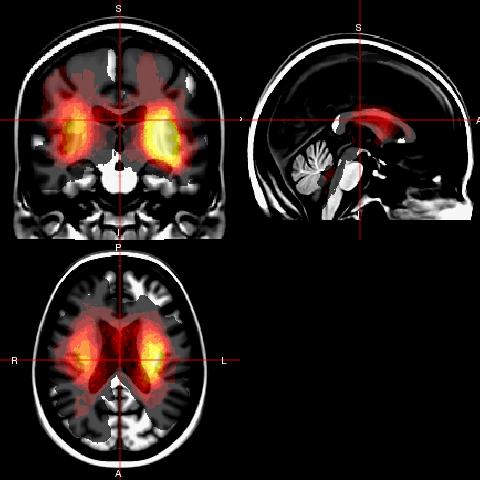
\includegraphics[width=.48\textwidth]{reoriented_Binary_Sum_Image_t1_heat_overlay.png}
}

\caption{{\bf ICH engagement prevalence.} The proportion of patients with ICH engaging a given voxel are represented in a 3D histogram (right side of image is left side of brain) overlaid on an MRI T1 template. There is a higher prevalence of ICH on the left side of the brain, localized in the middle of the brain, with few extensions in the anterior and posterior areas. The interactive version of this figure is located at \url{http://muschellij2.github.io/CT_Pipeline/index.html}.}
  \label{fig:StrokeHist}
\end{figure}

\ifseverity
\begin{figure}[H]
\centering
  \hfill
  \subfloat{
 \label{pvals:nihss}
 }
  \hfill
  \subfloat{
 \label{pvals:gcs}
 } 
 \newline
  \hfill
  \subfloat{
 \label{pvals:regnihss}
 }
  \hfill
  \subfloat{
 \label{pvals:reggcs}
 } 
 \newline 
  \caption{{\bf Highest Predictive Region (HPR) Analysis.}  Panels~\protect\subref{pvals:nihss} and~\protect\subref{pvals:gcs} correspond to the HPR for the top-performing model for NIHSS and GCS scores.  The HPR in \protect\subref{pvals:nihss} represents a p-value threshold of $.0100$ ($19047$ voxels) for the voxel-wise p-value of ICH on NIHSS. The HPR in \protect\subref{pvals:gcs} represents $1000$ with the lowest p-values for the voxel-wise ICH on GCS score regressions.
    Panels~\protect\subref{pvals:regnihss} and~\protect\subref{pvals:reggcs} plot the relationship of the HPR coverage and severity score.  The red line represents a linear fit, the blue line--a LOESS fit.  The larger the HPR coverage the higher (more severe) the NIHSS and the lower (deeper unconsciousness) the GCS.
}
  \label{f:roi}
\end{figure}
\fi

\newpage

\section*{Tables}


%% latex table generated in R 3.2.2 by xtable 1.8-0 package
% Fri Jan 29 01:56:29 2016
\begin{table}[ht]
\centering
\begin{tabular}{lc}
  \hline { Variable (N=111)} & { N (\%) or Mean (SD)} \\ 
  \hline
Age in Years: Mean (SD) & 60.8 (11.2) \\ 
   \hline
Female & 35 (31.5\%) \\ 
   \hline
ICH Volume: Mean (SD) & 37.4 (20.1) \\ 
   \hline
IVH Volume: Mean (SD) & 3.2 (6.3) \\ 
   \hline
Reader-Classified ICH Location &  \\ 
   \hline
\text{  } Putamen & 68 (61.3\%) \\ 
   \hline
\text{  } Lobar & 33 (29.7\%) \\ 
   \hline
\text{  } Globus Pallidus & 6 (5.4\%) \\ 
   \hline
\text{  } Thalamus & 4 (3.6\%) \\ 
   \hline
\end{tabular}
\caption{} 
\label{t:dem}
\end{table}









%% latex table generated in R 3.2.2 by xtable 1.8-0 package
% Fri Jan 29 01:56:30 2016
\begin{table}[ht]
\centering
\begin{tabular}{lccc}
  \hline
Area & Population Prevalence & NIHSS HPR & GCS HPR \\ 
  \hline
CSF (ventricular \& subarachnoid spaces) & 7.9 & 10.0 & 4.2 \\ 
  Insula & 4.7 &  &  \\ 
  Superior temporal gyrus & 3.8 &  &  \\ 
  Putamen left & 3.0 &  &  \\ 
  Insular right & 2.9 &  &  \\ 
  External capsule left & 2.3 &  &  \\ 
  Superior corona radiata left & 1.9 & 11.8 & 27.9 \\ 
  Superior temporal wm left & 1.9 &  &  \\ 
  Superior corona radiata right & 1.8 &  &  \\ 
  Putamen right & 1.8 &  &  \\ 
  Posterior limb of internal capsule left &  & 10.1 & 3.9 \\ 
  Thalamus left &  & 7.6 & 33.9 \\ 
  Caudate nucleus left &  & 5.4 & 9.6 \\ 
  Superior longitudinal fasciculus left &  & 4.9 & 5.9 \\ 
  Globus pallidus left &  & 3.7 &  \\ 
  Anterior limb of internal capsule left &  & 3.6 &  \\ 
  Outside brain mask &  & 3.5 &  \\ 
  Anterior limb of internal capsule right &  & 3.0 &  \\ 
  Postcentral wm left &  &  & 6.7 \\ 
  Posterior corona radiata left &  &  & 3.1 \\ 
  Precentral wm left &  &  & 1.3 \\ 
  Supramarginal wm left &  &  & 1.1 \\ 
   \hline
\end{tabular}
\caption{Percent engagement of the 3D histogram and top-performing HPR for the top 10 areas of engagement} 
\label{t:breakdown}
\end{table}

% latex table generated in R 3.2.2 by xtable 1.8-0 package
% Fri Jan 29 01:56:31 2016
\begin{table}[ht]
\centering
\begin{tabular}{lc}
  \hline
Area & Population Prevalence \\ 
  \hline
CSF (ventricular \& subarachnoid spaces) & 7.9 \\ 
  Insular & 7.6 \\ 
  Superior temporal gyrus & 5.5 \\ 
  Putamen & 4.8 \\ 
  External capsule & 3.9 \\ 
  Superior corona radiata & 3.7 \\ 
  Precentral gyrus & 3.3 \\ 
  Precentral WM & 3.1 \\ 
  Superior temporal WM & 3.1 \\ 
  Posterior limb of internal capsule & 3.0 \\ 
   \hline
\end{tabular}
\caption{{\bf Distribution of the Top 10 Areas of Engagement of Highest Predictive Regions.}} 
\label{t:breakdown}
\end{table}





\clearpage
\newpage

\section*{Figures}

\setcounter{figure}{0}

%
%\begin{figure}[H]
%\centering
%  \subfloat[\textbf{Distribution} of proportion of patients with hemorrhage. All voxels with 0 proportion are excluded.]{
%  \label{prop:hist}
%  \includegraphics[width=.48\textwidth]{reoriented_Binary_Sum_Image_histogram.pdf}
%}
%  \subfloat[\textbf{Template brain (MRI T1)} with proportion of hemorrhage overlaid]{
%  \label{prop:img}
%\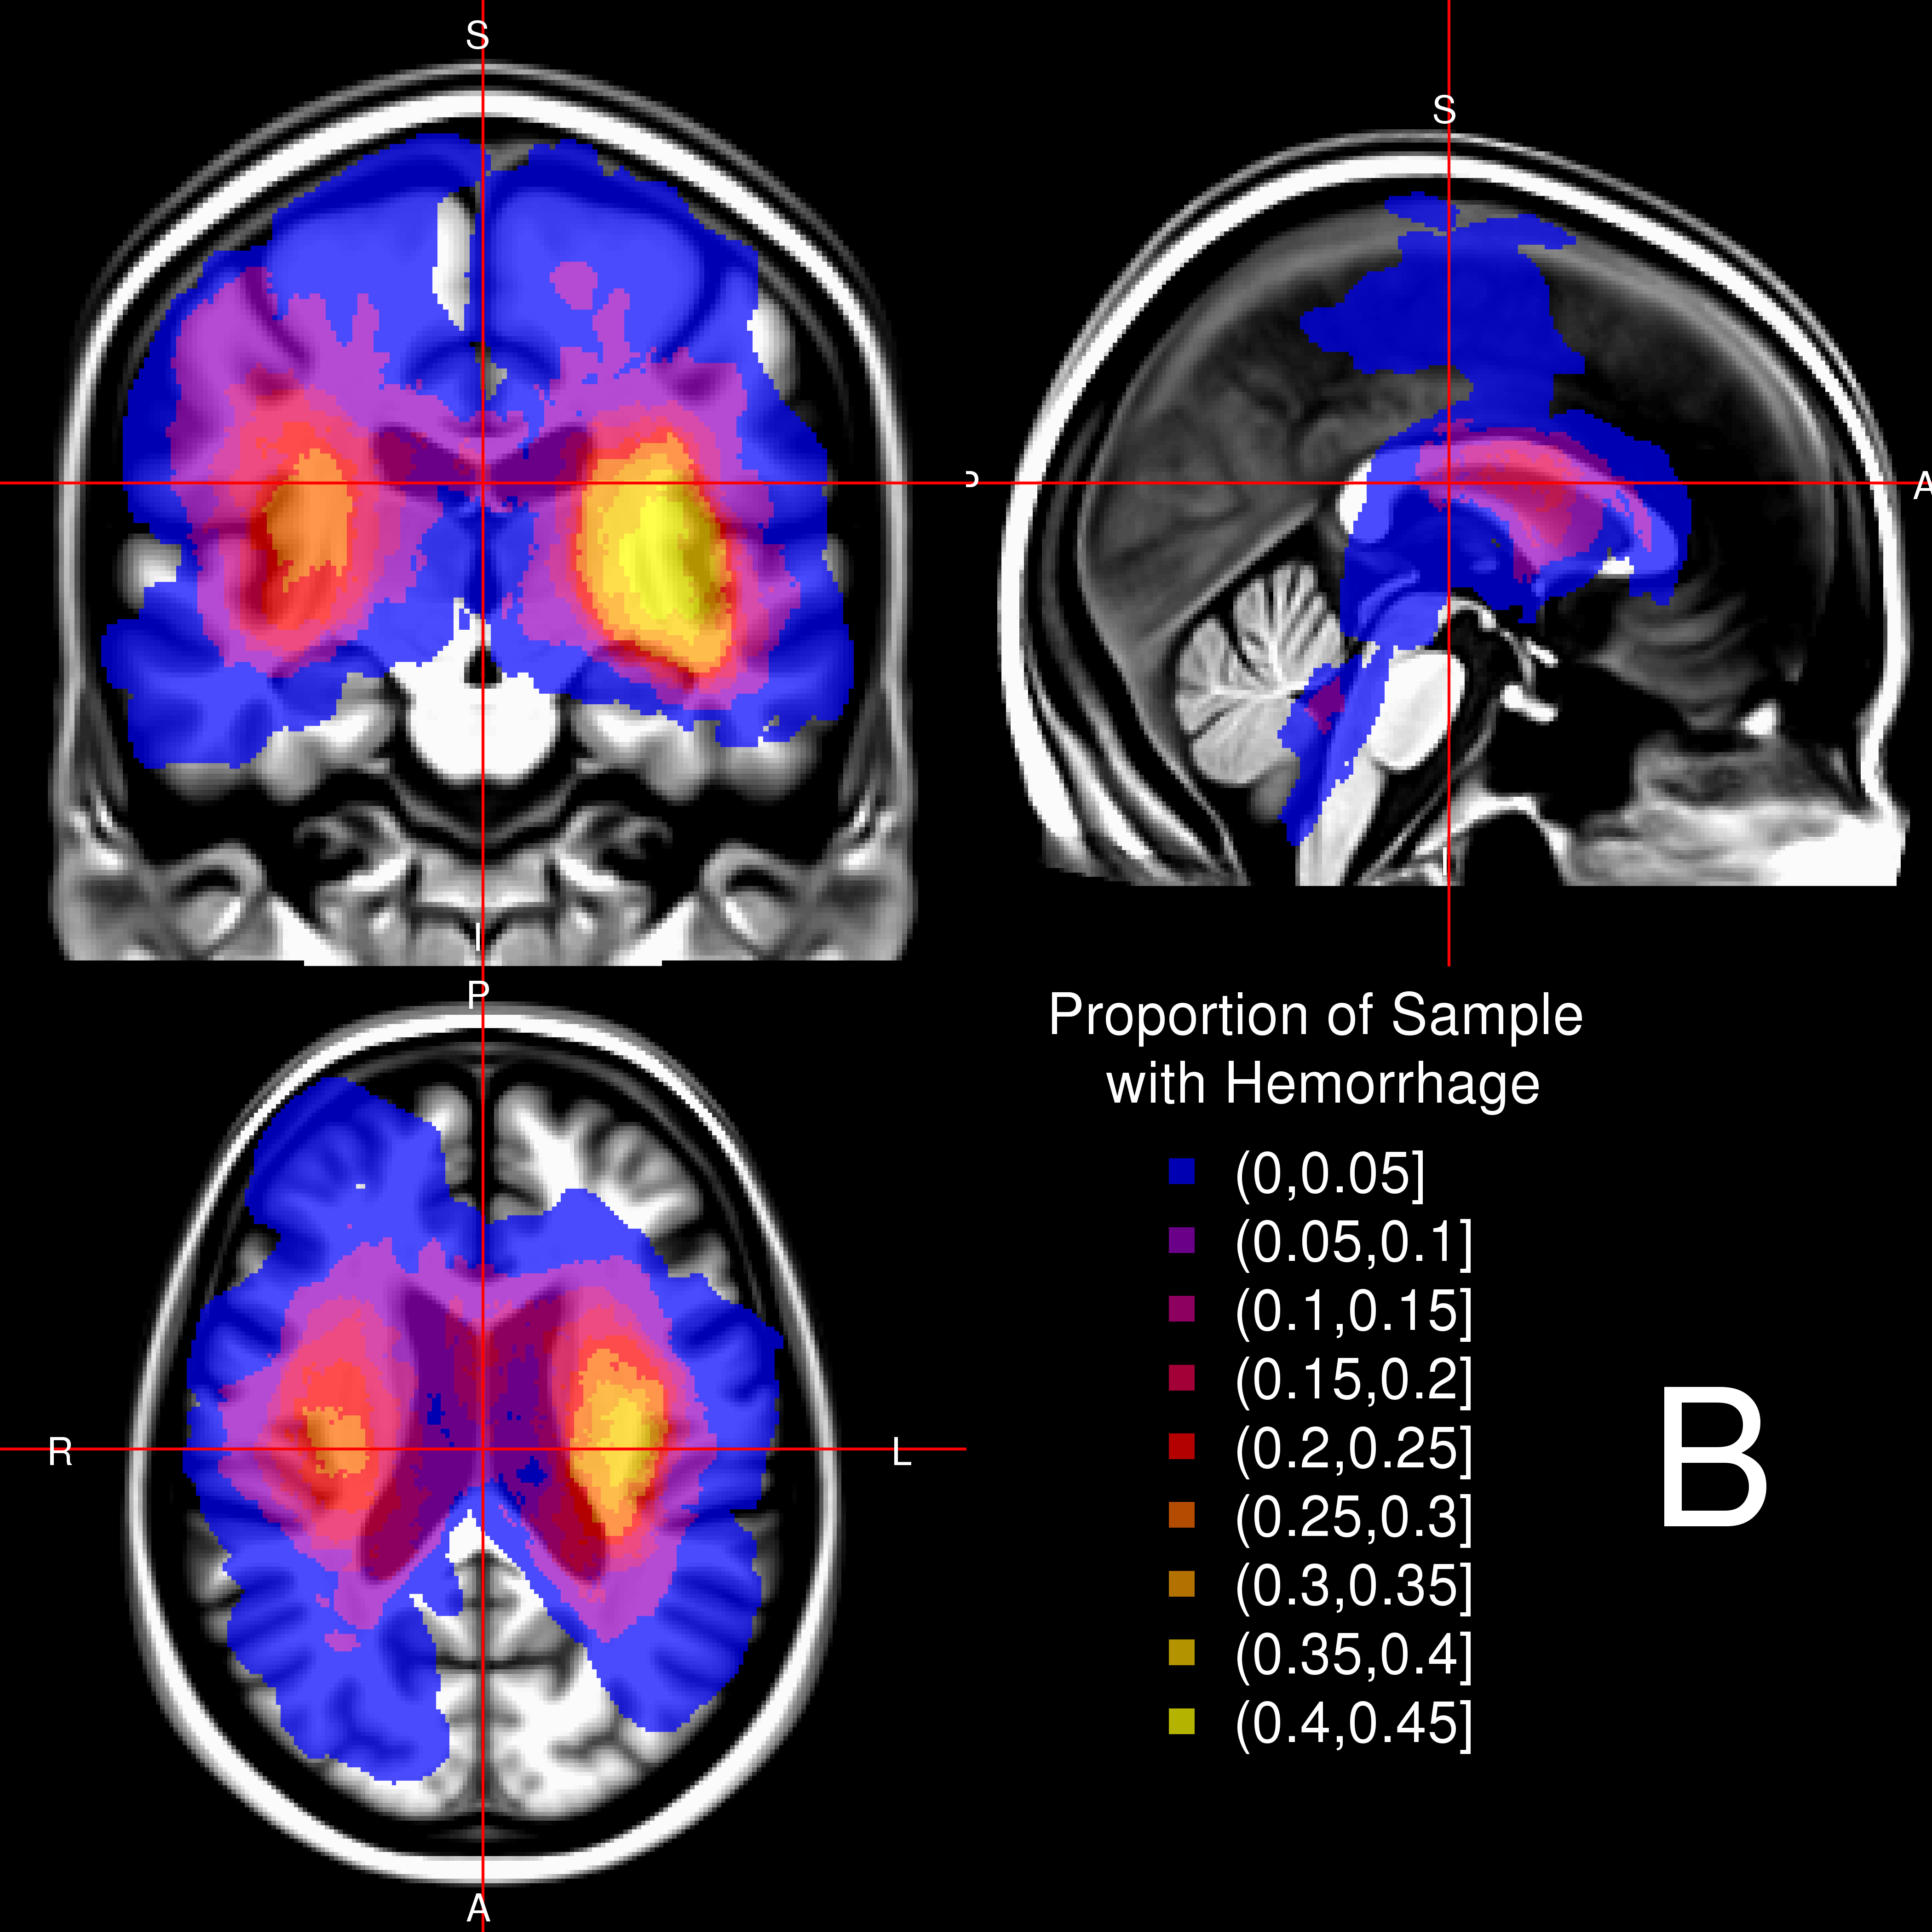
\includegraphics[width=.48\textwidth]{Figure4_Proportion.png}
%}
%  \label{fig:StrokeHist_old}
%\end{figure}

\begin{figure}[H]
\centering
  \subfloat{
	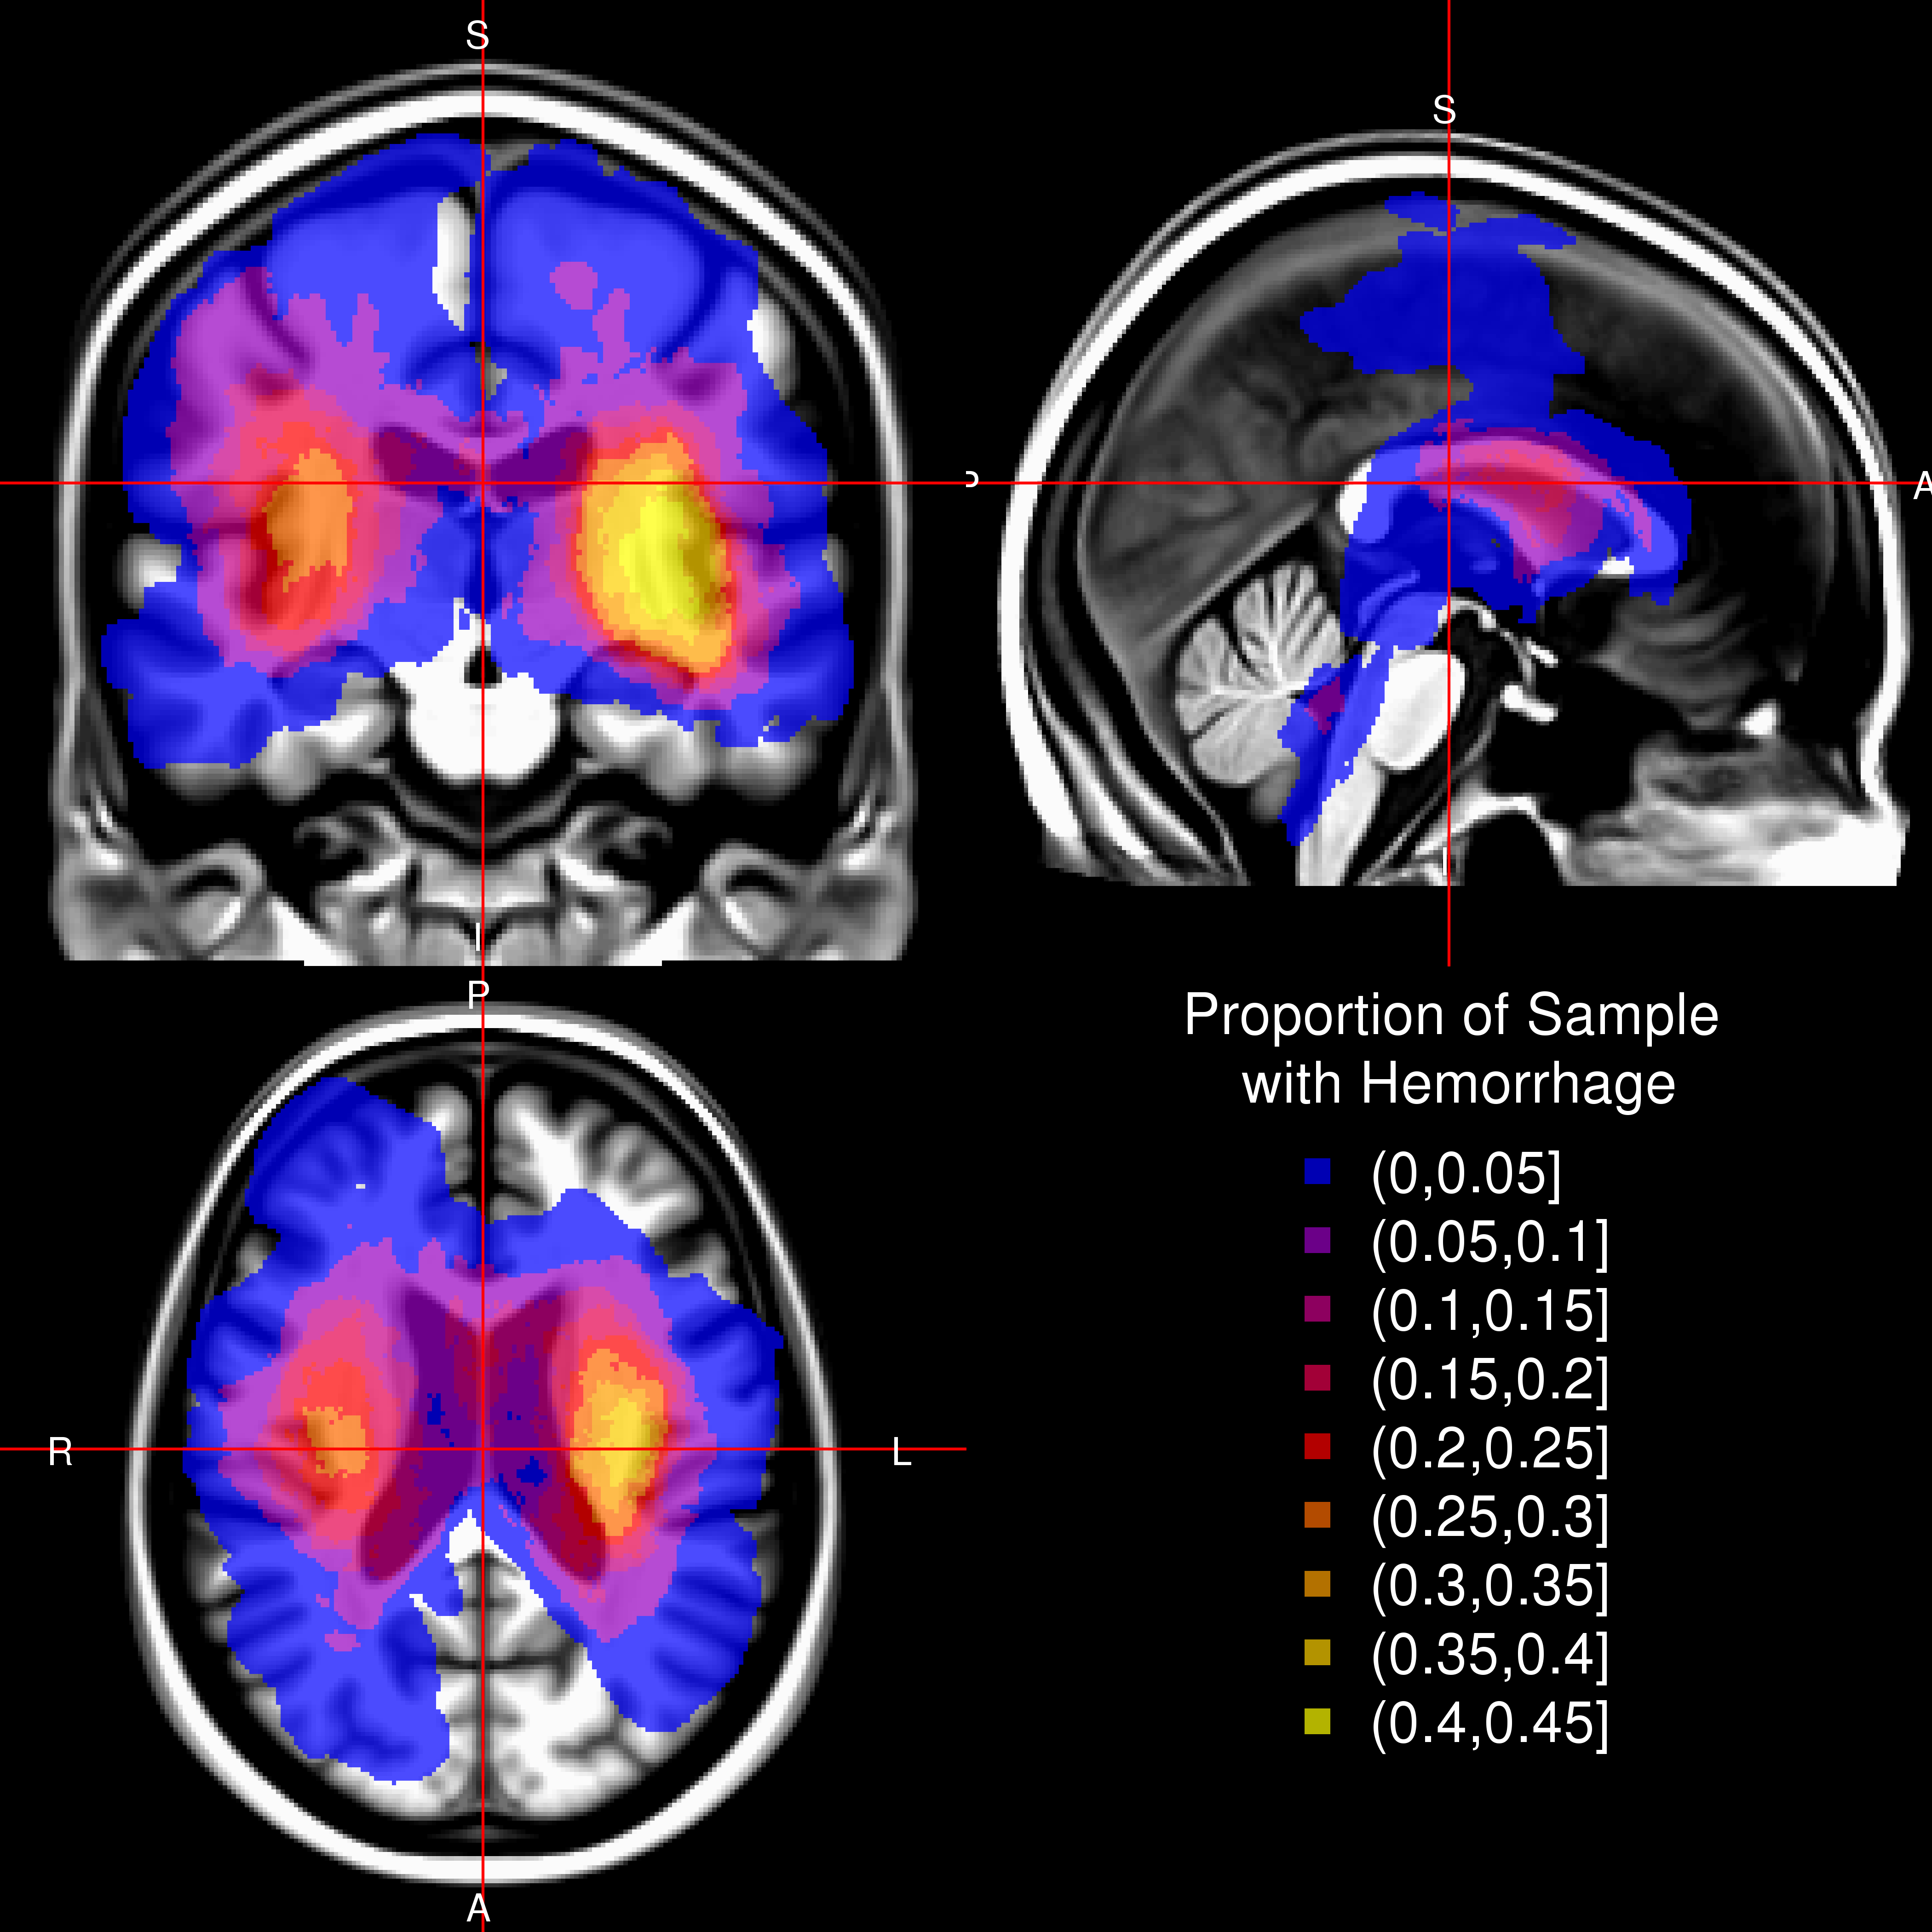
\includegraphics[width=.98\textwidth]{Figure4_Proportion_Final.png}
}
\caption{}
\end{figure}


\begin{figure}[H]
\centering
  \hfill
  \subfloat{
 \includegraphics[width=.48\textwidth]{{Top_0.01_pvalues_Final}.png}
 }
  \hfill
  \subfloat{
 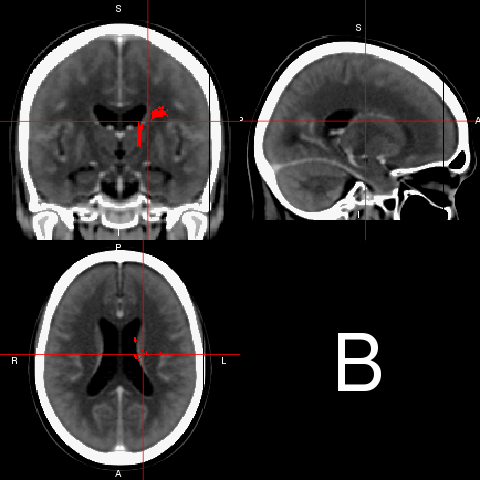
\includegraphics[width=.48\textwidth]{GCS_Top_1000_pvalues_Final.png}
 } 
 \newline
  \hfill
  \subfloat{
 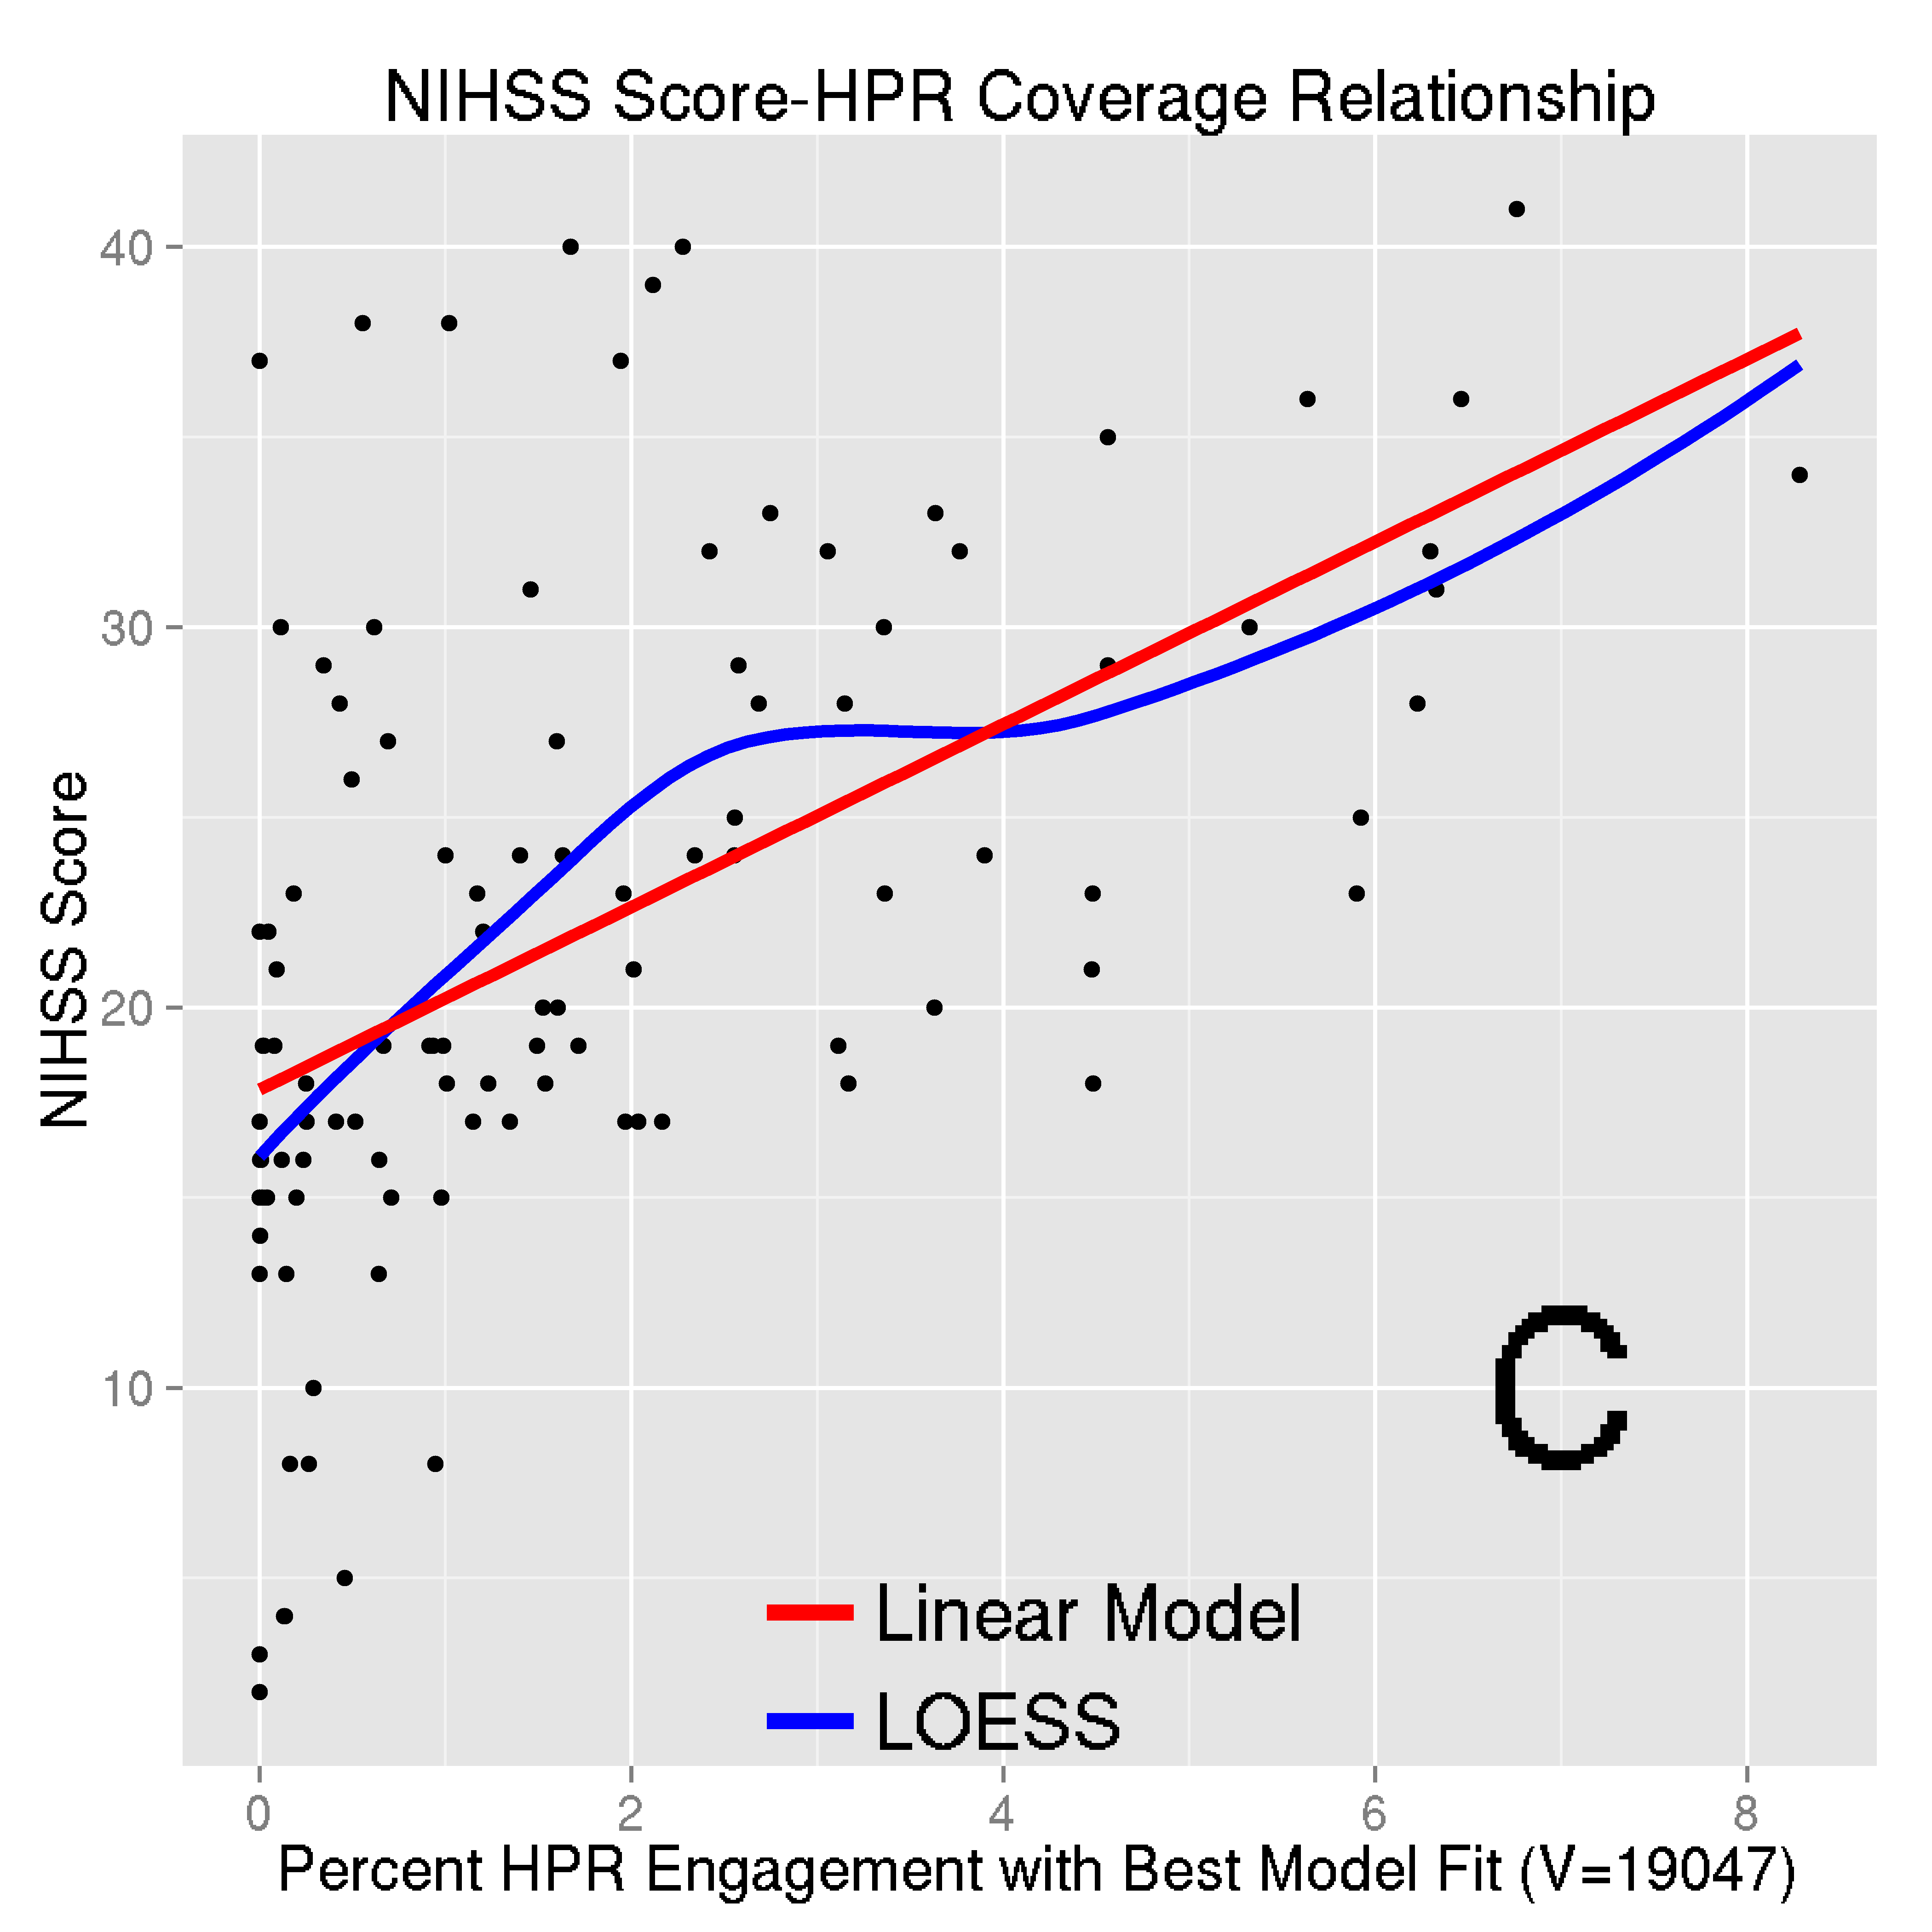
\includegraphics[width=.48\textwidth]{Regress_ROI_NIHSS_Best_Model.png}
 }
  \hfill
  \subfloat{
 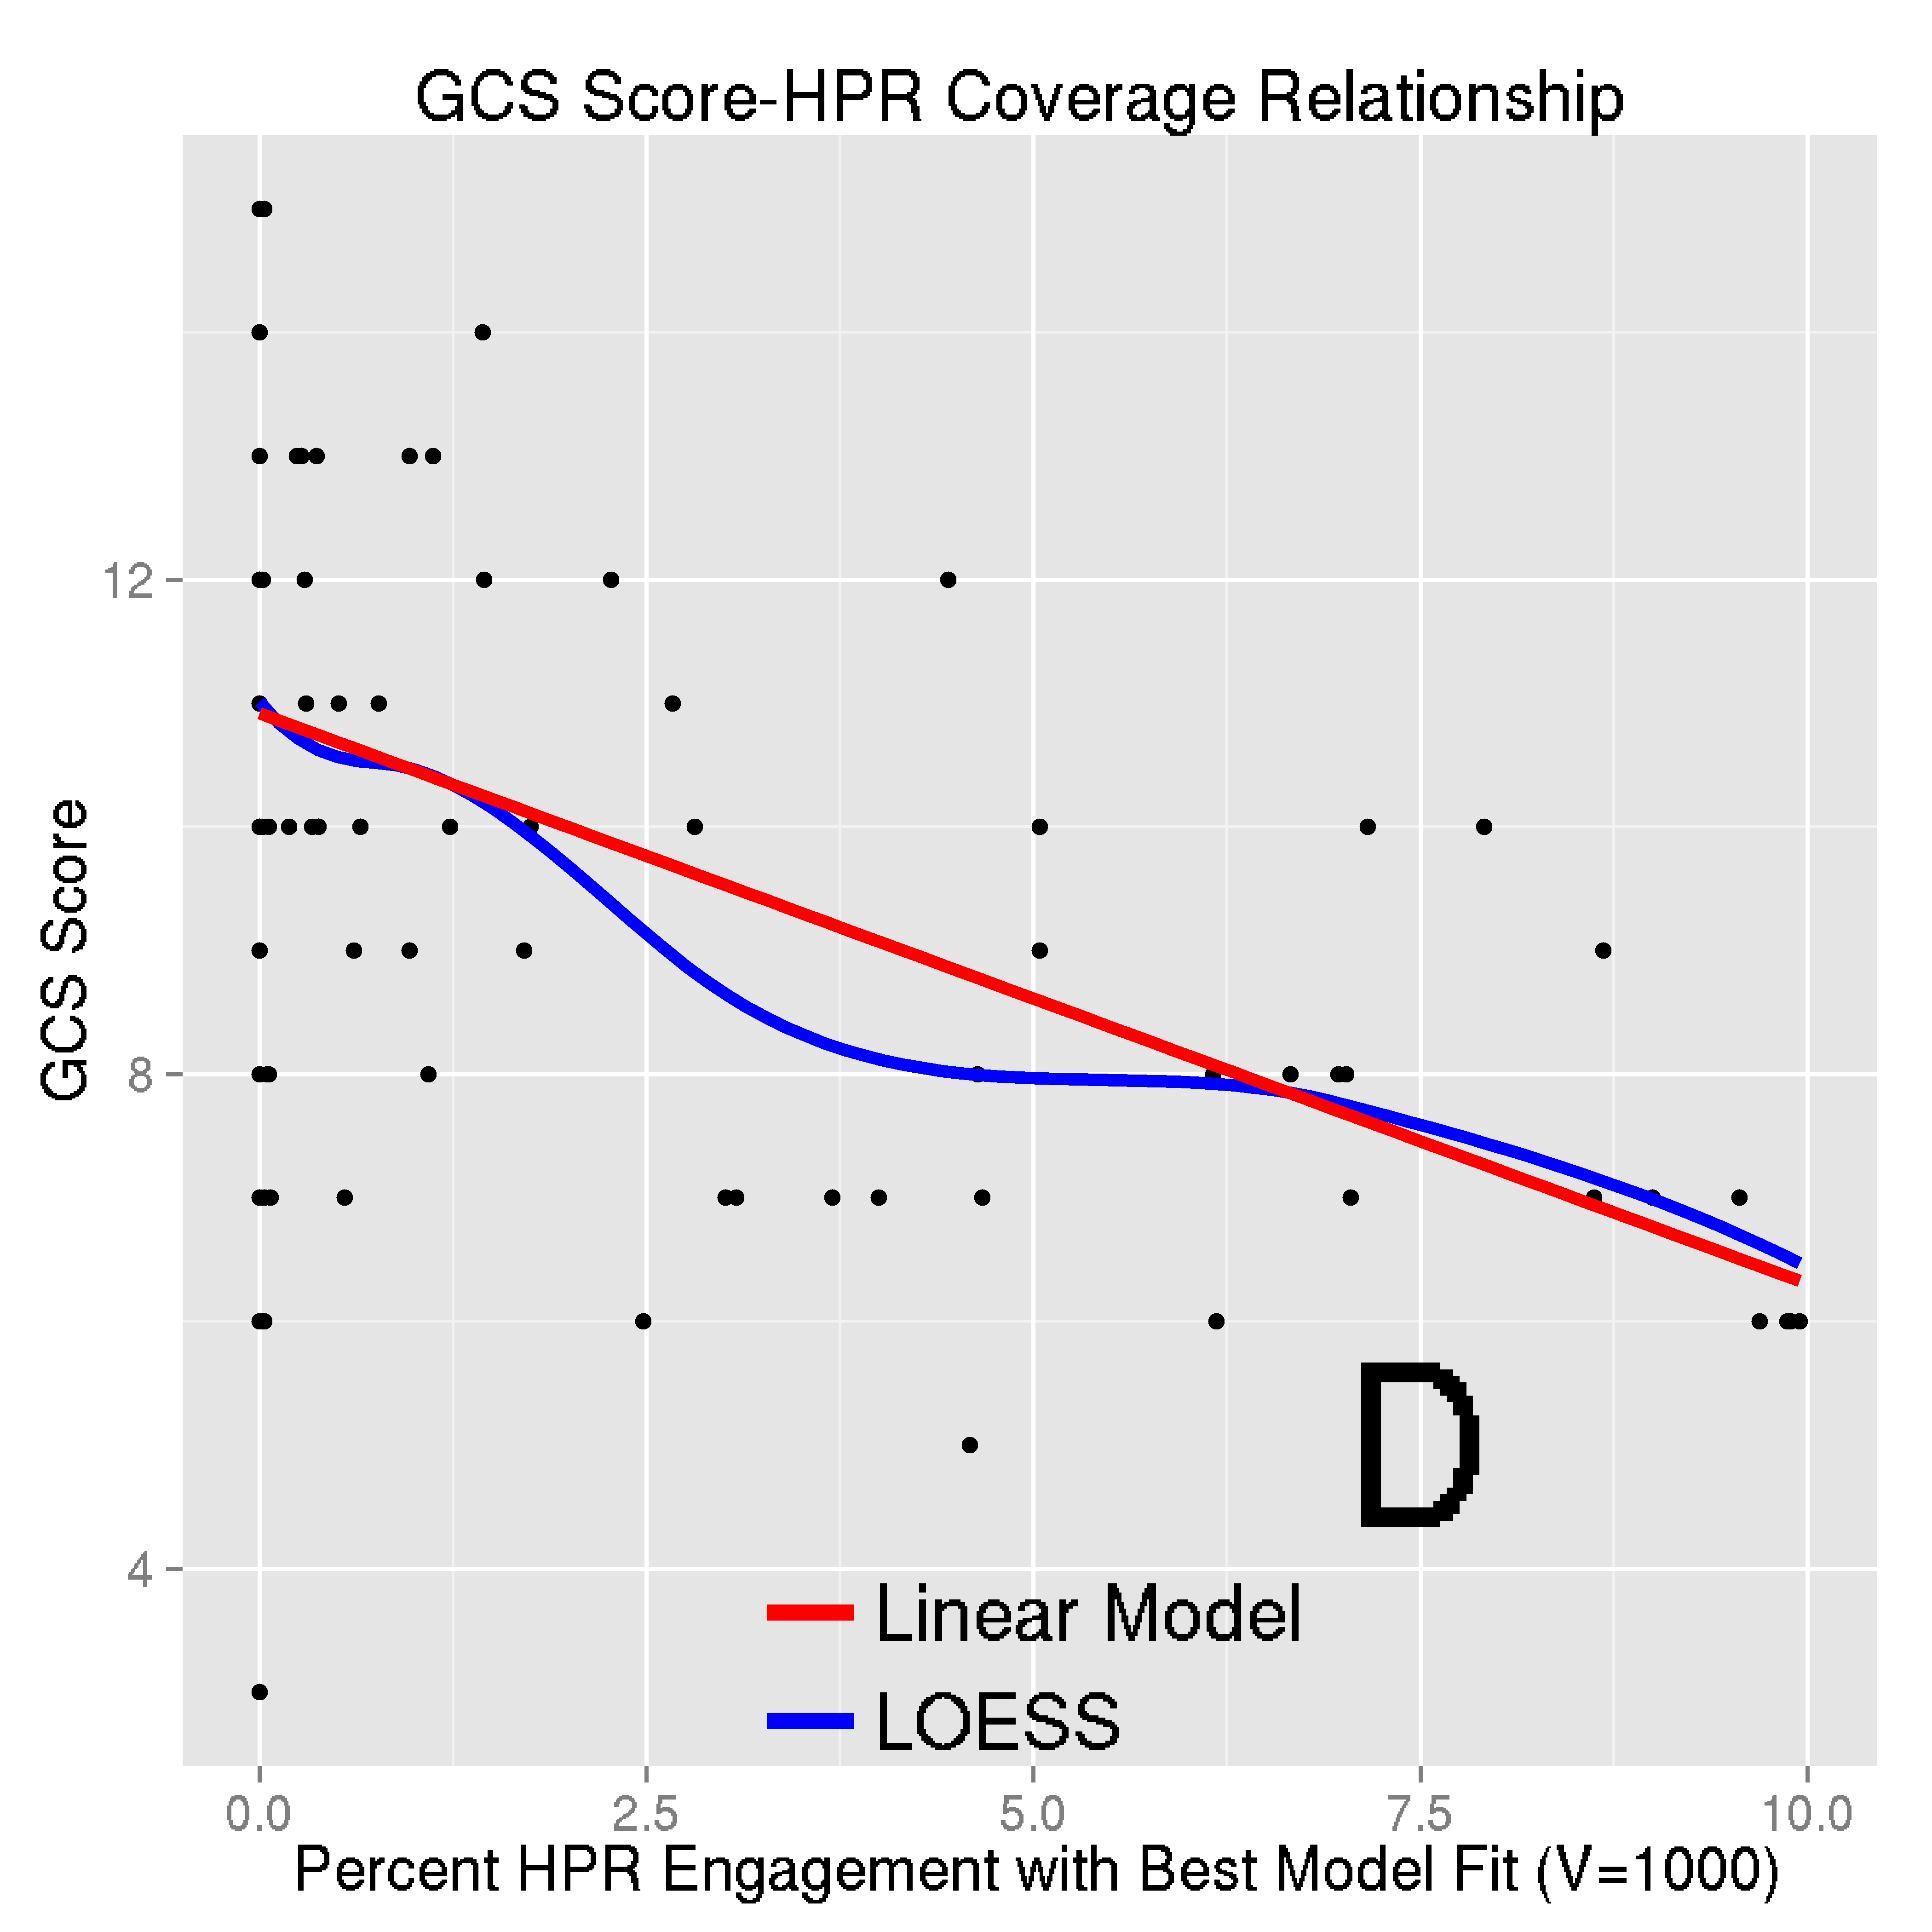
\includegraphics[width=.48\textwidth]{Regress_ROI_GCS_Best_Model.png}
 }  
 \caption{}
\end{figure}





\clearpage
\newpage

\thispagestyle{empty}
\pagestyle{plain}

\setcounter{figure}{0}
\renewcommand{\thefigure}{\Roman{figure}}
\setcounter{table}{0}
\renewcommand{\thetable}{\Roman{table}}

%\begin{refsection}
%
%
%\section*{Supplemental Material}
%\subsection*{Supplemental Methods}
%\subsubsection*{Image Processing: Brain Extraction, Reorientation, Registration}
%\label{sec:processing}
%The hemorrhage was excluded when registering the CT scan to the template using manual ICH segmentations.  Binary ICH masks had voxel values of $1$ if the voxel was hemorrhage, and $0$ otherwise.  
%
%The CT images were processed as follows:
%\begin{enumerate}
%\item Export from OsiriX to DICOM format
%\item Gantry tilt corrected (if applicable) using MATLAB script (\url{http://bit.ly/1ltIM8c})
%\item Converted to the Neuroimaging Informatics Technology Initiative (NIfTI) format using \verb|dcm2nii| (2009 version, MRIcro \citep{rorden_stereotaxic_2000})
%\item Brain extraction tool (BET) \citep{smith_fast_2002}, a function of FSL (v5.0.4) \citep{jenkinson_fsl_2012} was applied
%\item The data was aligned to the anterior-posterior commissure line (\url{http://bit.ly/1gUqMDw}).
%\item The Clinical MATLAB toolbox \citep{rorden_age-specific_2012} transformed the image and mask into template space.
%\end{enumerate}
% An image with its brain-extracted counterpart is displayed in Supplemental Figure~\ref{f:reg}\protect\subref*{reg:ss1}.
%
%We thresholded the registered-to-template hemorrhage mask: let $S_i$ be the mask for person $i$, and $s_{ij}$ be the intensity of voxel $j$ of that mask; let $v_{ij}$ represents voxel $j$ of the thresholded image.  The was thresholded using the rule \citep{rorden_age-specific_2012}:
%$$
%v_{ij} =
%\begin{cases}
%1  & \text{if } s_{ij} \geq \frac{\min(S_i) + \max(S_i)}{2}\\
%0  & \text{if } s_{ij} < \frac{\min(S_i) + \max(S_i)}{2}
%\end{cases}
%$$
%These binary ICH masks were used in analysis.  
%
%\subsubsection*{Calculating Region Engagement from the Eve Atlas}
%\label{sec:calc_perc}
%We also calculated the percent engagement of regions for the best-performing HPR for the NIHSS and GCS score analyses.
%More explicitly, let $k$ denote the brain region (e.g.~putamen) and let $\sum_{k} v_{k}$ represent the sum of the voxels for an image (HPR or population ICH image) in that brain region. These $p_{k}$ represent the percent that brain region engages the ICH compared to other regions (Table~\ref{t:breakdown}):
%$$
%  p_{k} = \frac{\sum_{k} v_{k}}{\text{Sum of Voxels in Analysis}}
%$$
%We also calculated brain region engagement with the population ICH or HPR images (Table~\ref{t:area_breakdown}):
%$$
%	r_{k} = \frac{\sum_{k} v_{k}}{\# \text{Number of Voxels in Region}}
%$$
%These percentages ($r_{k}$) are at a region level; $p_k$ are at an image level.
%
%
%
%\subsubsection*{Image Registration}
%
%
%We present the registration results (Figure~\ref{f:reg}):  manually segmented blood in the original space with the hemorrhage mask in pink (panel~\protect\subref*{reg:nat1}), brain-extracted image (panel~\protect\subref*{reg:ss1}), registered image and hemorrhage mask in template space (panel~\protect\subref*{reg:co1}), and the ICH mask on the template (panel~\protect\subref*{reg:temp1}).  These images represent one patient with variable slice thickness with a large hemorrhage.
%
%Though variable slice thickness is present, the transformation morphs the image into the full space of the template; therefore, non-linear registration seems to reasonably account for variable slice thickness, likely by non-uniform scaling.
%Gross brain features remain relatively unchanged, but large deformations of tissue, due to ICH, appear well preserved by registration.  
%
%%[Figure~\ref{f:reg}]
%
%
%
%\newpage
%
%\subsection*{Supplemental Tables}
%% latex table generated in R 3.2.2 by xtable 1.8-0 package
% Fri Jan 29 01:56:31 2016
\begin{table}[ht]
\centering
\begin{tabular}{lccc}
  \hline
Area & Population Engagement & NIHSS HPR & GCS HPR \\ 
  \hline
Globus Pallidus: Total & 20.3 & 40.0 & 0.0 \\ 
  Globus Pallidus: Right & 14.8 & 34.8 & 0.0 \\ 
  Globus Pallidus: Left & 25.2 & 44.7 & 0.0 \\ 
  Putamen: Total & 23.3 & 6.6 & 0.0 \\ 
  Putamen: Right & 17.5 & 3.8 & 0.0 \\ 
  Putamen: Left & 29.2 & 9.4 & 0.0 \\ 
  Thalamus: Total & 7.9 & 8.9 & 1.7 \\ 
  Thalamus: Right & 6.8 & 3.1 & 0.0 \\ 
  Thalamus: Left & 9.1 & 14.6 & 3.4 \\ 
   \hline
\end{tabular}
\caption{Thalamus, Putamen and Globus Pallidus ICH Engagement by the population and NIHSS/GCS HPR} 
\label{t:area_breakdown}
\end{table}

%
%
%\subsection*{Supplemental Figures and Figure Legends}
%
%
%\begin{figure}[H]
%\centering
% \subfloat{
% \includegraphics[width=.48\textwidth]{native_100-362_20100126_1926_CT_2_CT_ROUTINE.png}
% \label{reg:nat1}
% }
% \hfill
% \subfloat{
%% \includegraphics[width=.48\textwidth]{{100-362_20100126_1926_CT_2_CT_ROUTINE_SS_0.01}.png}
% \includegraphics[width=.48\textwidth]{ss_100-362_20100126_1926_CT_2_CT_ROUTINE.png}
% \label{reg:ss1}
%} 
%\newline
% \subfloat{
% \includegraphics[width=.48\textwidth]{raw_100-362_20100126_1926_CT_2_CT_ROUTINE.png}
% \label{reg:co1}
%}
%  \hfill
%  \subfloat{
% \includegraphics[width=.48\textwidth]{roi_100-362_20100126_1926_CT_2_CT_ROUTINE.png}
% \label{reg:temp1}
%} 
%  \caption{{\bf Steps of Image Processing}.  The native space image \protect\subref{reg:nat1}, with hemorrhage overlaid (pink), shows variable slice thickness: the top of the brain has smaller voxel sizes than the bottom of the brain.  The brain-extracted image used for AC-PC alignment is in panel~\protect\subref{reg:ss1}. 
%The template-registered image \protect\subref{reg:co1} was transformed and scaled to size as the template.  We see that similar structures, such as the lateral ventricles, are observed on the same axial slice on the patient-level scan compared to the template image, which indicates adequate registration. Panel~\protect\subref{reg:temp1} shows the overlaid hemorrhage mask on the CT template.
%  }
%  \label{f:reg}
%\end{figure}
%
%
%\begin{figure}[H]
%\centering
%  \subfloat{
%	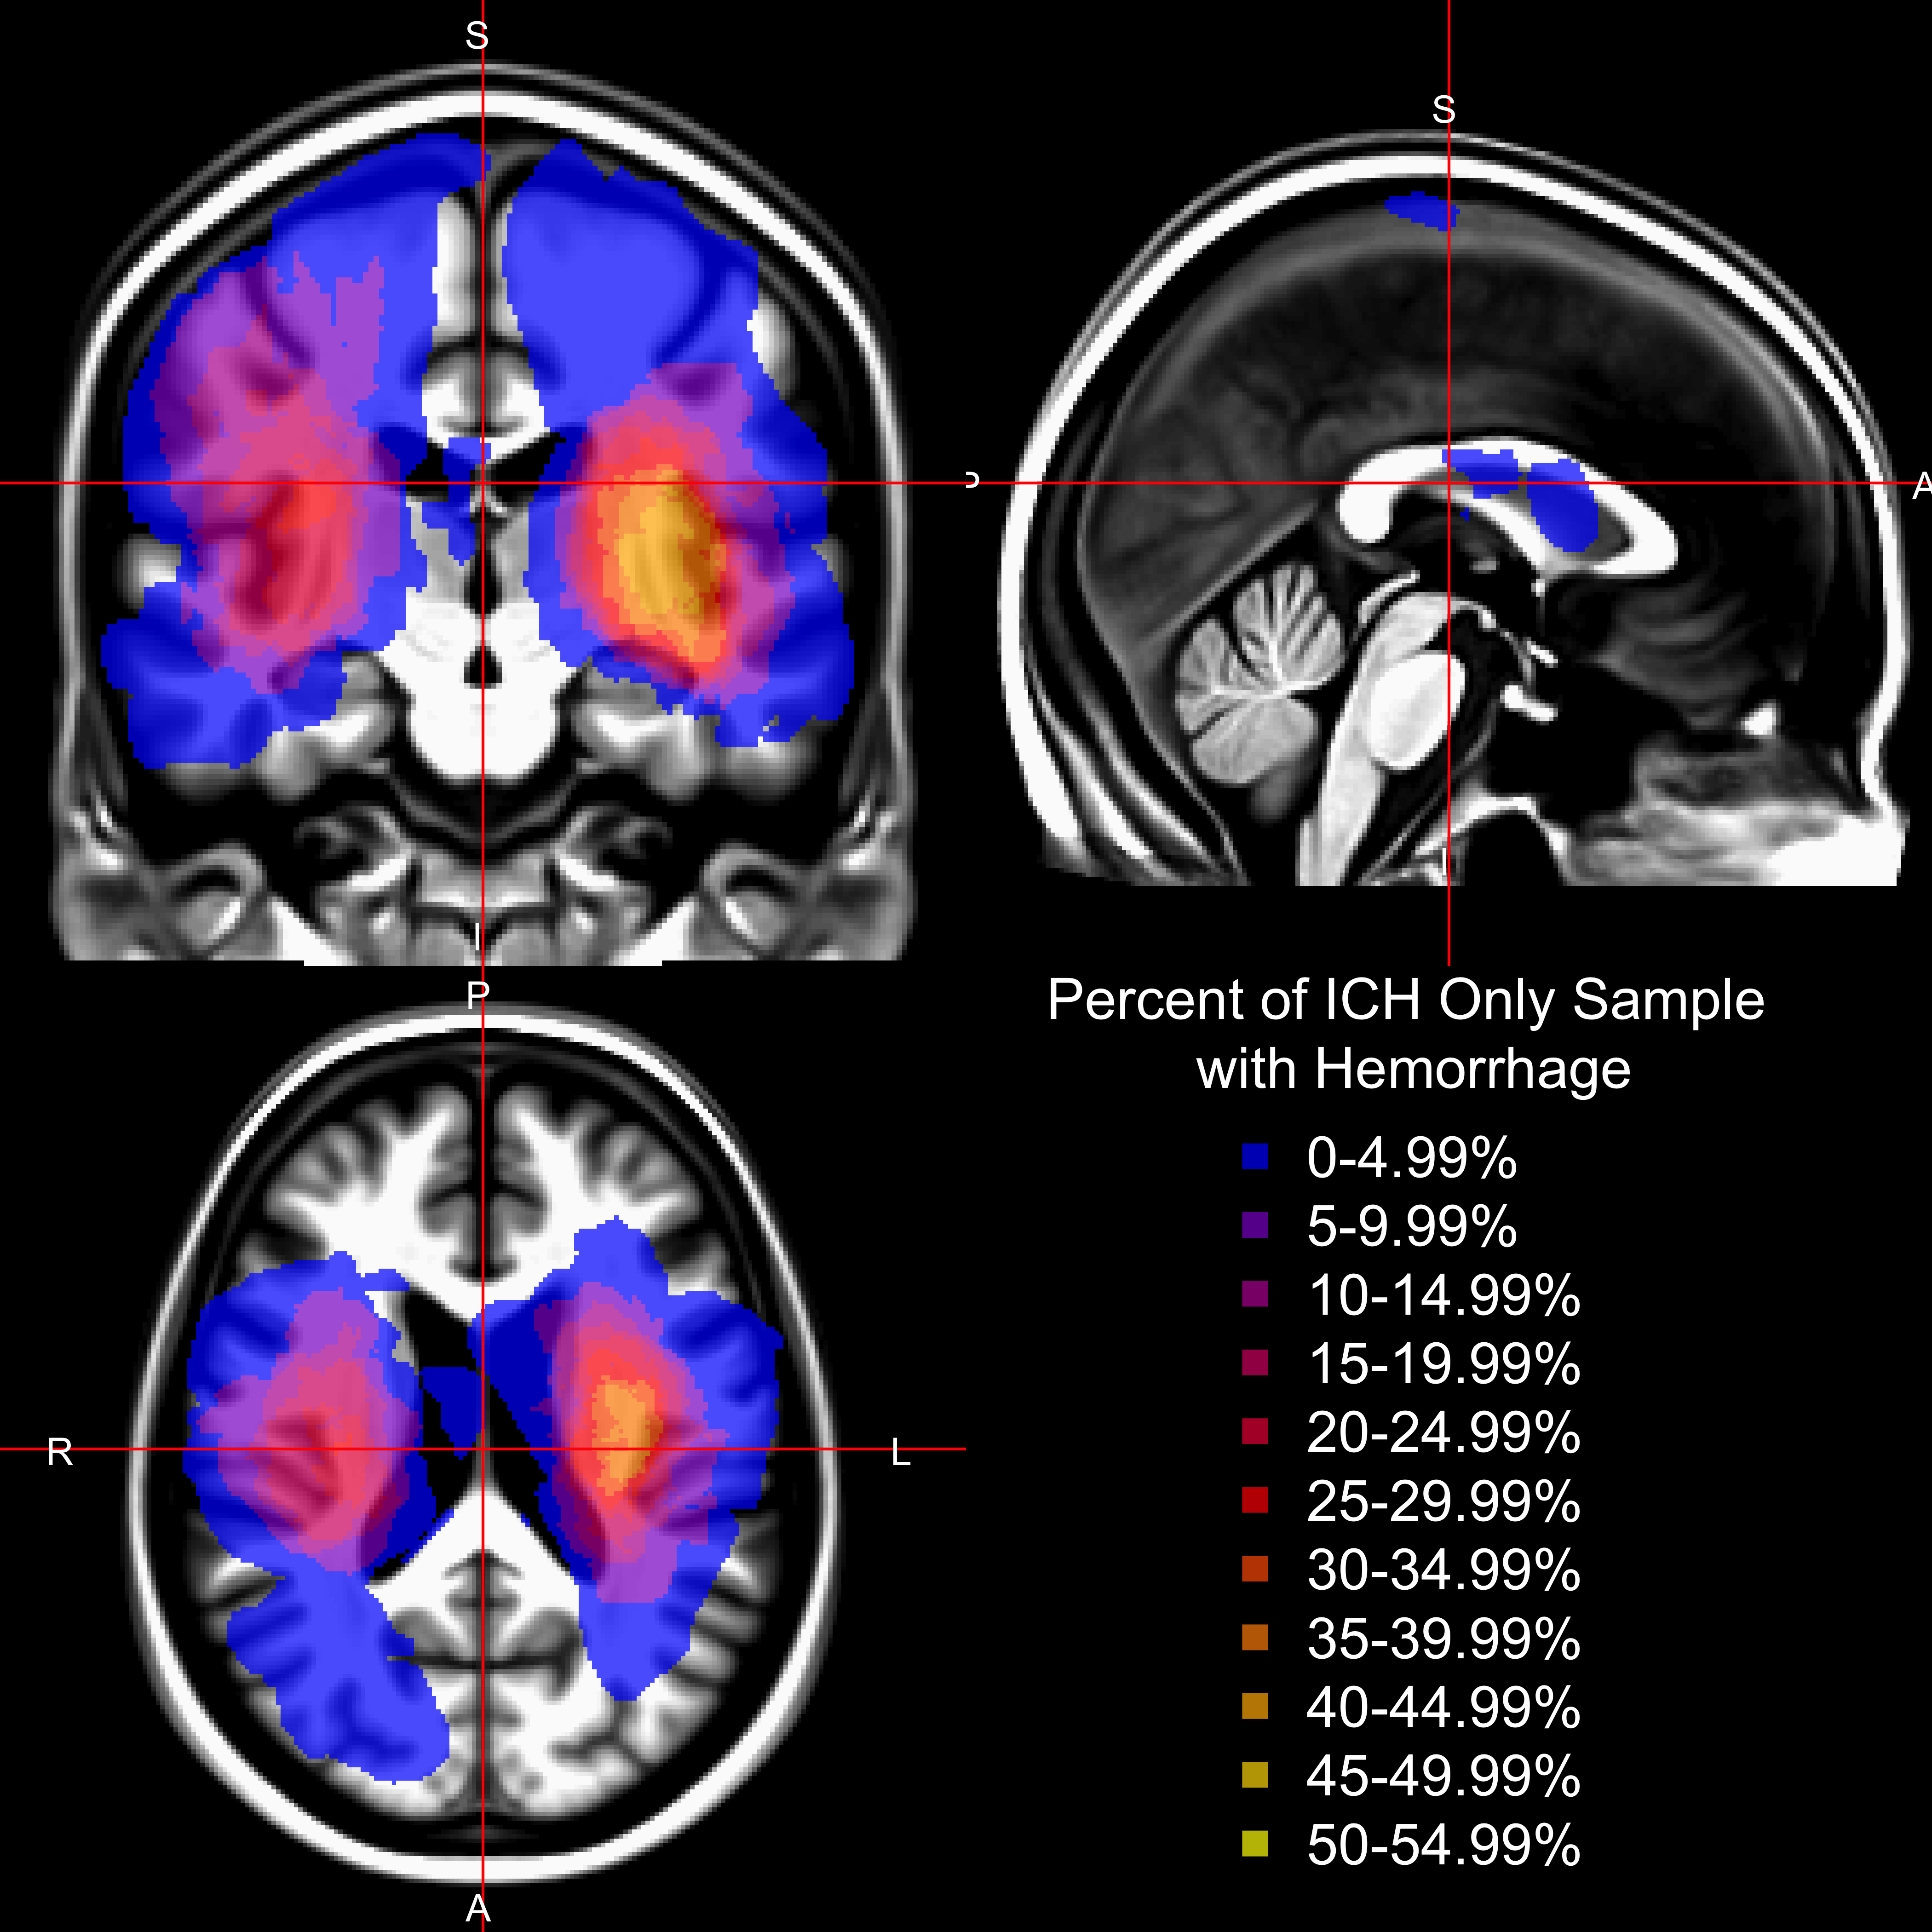
\includegraphics[width=.98\textwidth]{figure/Density_NoIVH.png}
%}
%\caption{{\bf ICH engagement prevalence in patients with no recorded IVH.} The proportion of patients with ICH, but without IVH, engaging a given voxel are represented in a 3D histogram (right side of image is left side of brain) overlaid on an MRI T1 template. Note that areas of the ventricles have a low prevalence (indicated by blue), indicating that much of the prevalence in the ventricular spaces the full population of images is due to IVH.
%}
%  \label{fig:StrokeHist_NoIVH}
%\end{figure}
%
%
%\clearpage
%\newpage
%\thispagestyle{empty}
%\pagestyle{plain}
%
%\printbibliography[title=Supplemental References]
%\end{refsection}




\end{document}

